\documentclass[12pt, a4paper]{report}
\usepackage{tikz}
\usepackage{standalone}
\usetikzlibrary{matrix,calc}

\newcommand{\implicantsol}[3][0]{
	\draw[rounded corners=3pt, fill=#3, opacity=0.3] ($(#2.north west)+(135:#1)$) rectangle ($(#2.south east)+(-45:#1)$);
}

\newcommand{\implicant}[4][0]{
	\draw[rounded corners=3pt, fill=#4, opacity=0.3] ($(#2.north west)+(135:#1)$) rectangle ($(#3.south east)+(-45:#1)$);
}

\newcommand{\implicantedges}[4][0]{
	\draw[rounded corners=3pt, fill=#4, opacity=0.3] ($(rf.east |- #2.north)+(90:#1)$)-| ($(#2.east)+(0:#1)$) |- ($(rf.east |- #3.south)+(-90:#1)$);
	\draw[rounded corners=3pt, fill=#4, opacity=0.3] ($(cf.west |- #2.north)+(90:#1)$) -| ($(#3.west)+(180:#1)$) |- ($(cf.west |- #3.south)+(-90:#1)$);
}


\newcommand{\implicanttopdown}[4][0]{
	\draw[rounded corners=3pt, fill=#4, opacity=0.3] ($(cf.south -| #2.west)+(180:#1)$) |- ($(#2.south)+(-90:#1)$) -| ($(cf.south -| #3.east)+(0:#1)$);
	\draw[rounded corners=3pt, fill=#4, opacity=0.3] ($(rf.north -| #2.west)+(180:#1)$) |- ($(#3.north)+(90:#1)$) -| ($(rf.north -| #3.east)+(0:#1)$);
}

\newcommand{\implicantcorners}[2][0]{
	\draw[rounded corners=3pt, opacity=.3] ($(rf.east |- 0.south)+(-90:#1)$) -| ($(0.east |- cf.south)+(0:#1)$);
	\draw[rounded corners=3pt, opacity=.3] ($(rf.east |- 8.north)+(90:#1)$) -| ($(8.east |- rf.north)+(0:#1)$);
	\draw[rounded corners=3pt, opacity=.3] ($(cf.west |- 2.south)+(-90:#1)$) -| ($(2.west |- cf.south)+(180:#1)$);
	\draw[rounded corners=3pt, opacity=.3] ($(cf.west |- 10.north)+(90:#1)$) -| ($(10.west |- rf.north)+(180:#1)$);
	\fill[rounded corners=3pt, fill=#2, opacity=.3] ($(rf.east |- 0.south)+(-90:#1)$) -|  ($(0.east |- cf.south)+(0:#1)$) [sharp corners] ($(rf.east |- 0.south)+(-90:#1)$) |-  ($(0.east |- cf.south)+(0:#1)$) ;
	\fill[rounded corners=3pt, fill=#2, opacity=.3] ($(rf.east |- 8.north)+(90:#1)$) -| ($(8.east |- rf.north)+(0:#1)$) [sharp corners] ($(rf.east |- 8.north)+(90:#1)$) |- ($(8.east |- rf.north)+(0:#1)$) ;
	\fill[rounded corners=3pt, fill=#2, opacity=.3] ($(cf.west |- 2.south)+(-90:#1)$) -| ($(2.west |- cf.south)+(180:#1)$) [sharp corners]($(cf.west |- 2.south)+(-90:#1)$) |- ($(2.west |- cf.south)+(180:#1)$) ;
	\fill[rounded corners=3pt, fill=#2, opacity=.3] ($(cf.west |- 10.north)+(90:#1)$) -| ($(10.west |- rf.north)+(180:#1)$) [sharp corners] ($(cf.west |- 10.north)+(90:#1)$) |- ($(10.west |- rf.north)+(180:#1)$) ;
}

%Empty Karnaugh map 4x4
\newenvironment{4kmap}[2]%
{
	\begin{tikzpicture}[baseline=(current bounding box.north),scale=0.8]
		\draw (0,0) grid (4,4);
		\draw (0,4) -- node [pos=0.7,above right,anchor=south west] {\tiny{#1}} node [pos=0.7,below left,anchor=north east] {\tiny{#2}} ++(135:1);
		%
		\matrix (mapa) [matrix of nodes,
		column sep={0.8cm,between origins},
		row sep={0.8cm,between origins},
		every node/.style={minimum size=0.3mm},
		anchor=8.center,
		ampersand replacement=\&] at (0.5,0.5)
		{
			\& |(c00)| 00         \& |(c01)| 01         \& |(c11)| 11         \& |(c10)| 10         \& |(cf)| \phantom{00} \\
			|(r00)| 00             \& |(0)|  \phantom{0} \& |(1)|  \phantom{0} \& |(3)|  \phantom{0} \& |(2)|  \phantom{0} \&                     \\
			|(r01)| 01             \& |(4)|  \phantom{0} \& |(5)|  \phantom{0} \& |(7)|  \phantom{0} \& |(6)|  \phantom{0} \&                     \\
			|(r11)| 11             \& |(12)| \phantom{0} \& |(13)| \phantom{0} \& |(15)| \phantom{0} \& |(14)| \phantom{0} \&                     \\
			|(r10)| 10             \& |(8)|  \phantom{0} \& |(9)|  \phantom{0} \& |(11)| \phantom{0} \& |(10)| \phantom{0} \&                     \\
			|(rf) | \phantom{00}   \&                    \&                    \&                    \&                    \&                     \\
		};
	}%
	{
	\end{tikzpicture}
}

%Empty Karnaugh map 2x4
\newenvironment{24kmap}[2]%
{
	\begin{tikzpicture}[baseline=(current bounding box.north),scale=0.8]
		\draw (0,0) grid (4,2);
		\draw (0,2) -- node [pos=0.7,above right,anchor=south west] {\tiny{#1}} node [pos=0.7,below left,anchor=north east] {\tiny{#2}} ++(135:1);
		%
		\matrix (mapa) [matrix of nodes,
		column sep={0.8cm,between origins},
		row sep={0.8cm,between origins},
		every node/.style={minimum size=0.3mm},
		anchor=4.center,
		ampersand replacement=\&] at (0.5,0.5)
		{
			\& |(c00)| 00         \& |(c01)| 01         \& |(c11)| 11         \& |(c10)| 10         \& |(cf)| \phantom{00} \\
			|(r00)| 0             \& |(0)|  \phantom{0} \& |(1)|  \phantom{0} \& |(3)|  \phantom{0} \& |(2)|  \phantom{0} \&                     \\
			|(r01)| 1             \& |(4)|  \phantom{0} \& |(5)|  \phantom{0} \& |(7)|  \phantom{0} \& |(6)|  \phantom{0} \&                     \\
			|(rf) | \phantom{00}  \&                    \&                    \&                    \&                    \&                     \\
		};
	}%
	{
	\end{tikzpicture}
}

%Empty Karnaugh map 2x2
\newenvironment{22kmap}%
{
	\begin{tikzpicture}[baseline=(current bounding box.north),scale=0.8]
		\draw (0,0) grid (2,2);
		\draw (0,2) -- node [pos=0.7,above right,anchor=south west] {b} node [pos=0.7,below left,anchor=north east] {a} ++(135:1);
		%
		\matrix (mapa) [matrix of nodes,
		column sep={0.8cm,between origins},
		row sep={0.8cm,between origins},
		every node/.style={minimum size=0.3mm},
		anchor=2.center,
		ampersand replacement=\&] at (0.5,0.5)
		{
			\& |(c00)| 0          \& |(c01)| 1  \\
			|(r00)| 0 \& |(0)|  \phantom{0} \& |(1)|  \phantom{0} \\
			|(r01)| 1 \& |(2)|  \phantom{0} \& |(3)|  \phantom{0} \\
		};
	}%
	{
	\end{tikzpicture}
}

%Defines 8 or 16 values (0,1,X)
\newcommand{\contingut}[1]{%
	\foreach \x [count=\xi from 0]  in {#1}
	\path (\xi) node {\x};
}

%Places 1 in listed positions
\newcommand{\minterms}[1]{%
	\foreach \x in {#1}
	\path (\x) node {1};
}

%Places 0 in listed positions
\newcommand{\maxterms}[1]{%
	\foreach \x in {#1}
	\path (\x) node {0};
}

%Places X in listed positions
\newcommand{\indeterminants}[1]{%
	\foreach \x in {#1}
	\path (\x) node {X};
}


\usepackage{textcomp}
\usepackage{multicol}
\usepackage{multirow}
\usepackage{graphicx}
\graphicspath{ {./images/} }

\usepackage[siunitx, RPvoltages]{circuitikz}
\usepackage[leqno]{amsmath}
\usepackage[most]{tcolorbox}
\usepackage{varwidth}   %% provides varwidth environmen
\usepackage{amsmath,empheq}
\usepackage{polynom}
\everymath{\displaystyle}
\makeatletter
\def\pld@CF@loop#1+{%
	\ifx\relax#1\else
	\begingroup
	\pld@AccuSetX11%
	\def\pld@frac{{}{}}\let\pld@symbols\@empty\let\pld@vars\@empty
	\pld@false
	#1%
	\let\pld@temp\@empty
	\pld@AccuIfOne{}{\pld@AccuGet\pld@temp
		\edef\pld@temp{\noexpand\pld@R\pld@temp}}%
	\pld@if \pld@Extend\pld@temp{\expandafter\pld@F\pld@frac}\fi
	\expandafter\pld@CF@loop@\pld@symbols\relax\@empty
	\expandafter\pld@CF@loop@\pld@vars\relax\@empty
	\ifx\@empty\pld@temp
	\def\pld@temp{\pld@R11}%
	\fi
	\global\let\@gtempa\pld@temp
	\endgroup
	\ifx\@empty\@gtempa\else
	\pld@ExtendPoly\pld@tempoly\@gtempa
	\fi
	\expandafter\pld@CF@loop
	\fi}
\def\pld@CMAddToTempoly{%
	\pld@AccuGet\pld@temp\edef\pld@temp{\noexpand\pld@R\pld@temp}%
	\pld@CondenseMonomials\pld@false\pld@symbols
	\ifx\pld@symbols\@empty \else
	\pld@ExtendPoly\pld@temp\pld@symbols
	\fi
	\ifx\pld@temp\@empty \else
	\pld@if
	\expandafter\pld@IfSum\expandafter{\pld@temp}%
	{\expandafter\def\expandafter\pld@temp\expandafter
		{\expandafter\pld@F\expandafter{\pld@temp}{}}}%
	{}%
	\fi
	\pld@ExtendPoly\pld@tempoly\pld@temp
	\pld@Extend\pld@tempoly{\pld@monom}%
	\fi}
\makeatother
\usepackage{gensymb}
\makeatletter
\let\savedchap\@makechapterhead
\def\@makechapterhead{\vspace*{-3cm}\savedchap}
\usepackage{amssymb}
\usepackage{setspace}
\usepackage[norndcorners,customcolors]{hf-tikz}
\tikzset{set border color=black,set fill color=white}
\newcommand*{\qe}{$x=\frac{-b\pm\sqrt{b^2-4ac}}{2a}$}
\usepackage[linewidth=1pt]{mdframed}
\usepackage{fancyhdr}
\pagestyle{fancy}
\fancyhf{}
\lhead{\leftmark}
\rfoot{\thepage}
\usepackage{array}

\usepackage[utf8]{inputenc}
\usepackage{chngcntr}
\usepackage[english]{babel}
\makeatletter
\newcommand{\leqnomode}{\tagsleft@true\let\veqno\@@leqno}
\newcommand{\reqnomode}{\tagsleft@false\let\veqno\@@eqno}
\makeatother
\usepackage{amsmath}
\newtheorem{example}{Example}
\newtheorem{exercise}{Exercise}
\counterwithin*{example}{section}
\counterwithin*{example}{subsection}
\usepackage{titling}
\newcommand*{\qed}{\null\nobreak\hfill\ensuremath{\square}}%
\predate{}
\postdate{}
\date{} % clear date
\usepackage{draftwatermark}
\setlength{\jot}{13pt}
\counterwithin*{example}{section}
\counterwithin*{example}{subsection}
\title{Computer Logic: Module 1}
\addtolength{\parskip}{-0.5mm}
\begin{document}
	\begin{titlepage} % Suppresses headers and footers on the title page
		
		\centering % Centre everything on the title page
		
		\scshape % Use small caps for all text on the title page
		
		\vspace*{\baselineskip} % White space at the top of the page
		
		%------------------------------------------------
		%	Title
		%------------------------------------------------
		
		\rule{\textwidth}{1.6pt}\vspace*{-\baselineskip}\vspace*{2pt} % Thick horizontal rule
		\rule{\textwidth}{0.4pt} % Thin horizontal rule
		
		\vspace{0.75\baselineskip} % Whitespace above the title
		
		{\LARGE Module 1: \\Computer Arithmetic and Logic} % Title
		
		\vspace{0.75\baselineskip} % Whitespace below the title
		
		\rule{\textwidth}{0.4pt}\vspace*{-\baselineskip}\vspace{3.2pt} % Thin horizontal rule
		\rule{\textwidth}{1.6pt} % Thick horizontal rule
		
		\vspace{2\baselineskip} % Whitespace after the title block
		
		%------------------------------------------------
		%	Subtitle
		%------------------------------------------------
		
		“Once your soul has been enlarged by a truth, it can never return to its original size.”\\
		-Blaise Pascal% Subtitle or further description
		
		\vspace*{3\baselineskip} % Whitespace under the subtitle
		
		%------------------------------------------------
		%	Editor(s)
		%------------------------------------------------
		
		Notes By
		
		\vspace{0.5\baselineskip} % Whitespace before the editors
		
		{\scshape\Large Giorgio Grigolo \\ } % Editor list
		
		\vspace{0.5\baselineskip} % Whitespace below the editor list
		
		\textit{Student of Mathematics and Computer Science \\St.Aloysius College } % Editor affiliation
		
		\vfill % Whitespace between editor names and publisher logo
		
		%------------------------------------------------
		%	Publisher
		%------------------------------------------------
		
		
		\vspace{0.3\baselineskip} % Whitespace under the publisher logo
		
		2020 % Publication year
		
	\end{titlepage}
	\tableofcontents
	\newpage
	\SetWatermarkText{Giorgio G.}
	\SetWatermarkScale{5}
	\part{Computer Arithmetic and Logic}
	\chapter{Computer Arithmetic}
	\section{Binary numbers}
	There are two types of binary numbers: 
	\begin{itemize}
		\item{Signed binary numbers}
		\subitem{This type of number hold a sign of magnitude.}
		\item{Unsigned binary numbers}
		\subitem{This type of number is regarded as positive.}
	\end{itemize}
	\subsection{Unsigned binary numbers}
	\begin{center}
		\begin{tabular}{cccccccc}
			MSB &    &    &    &   &   &   & LSB \\ \hline
			128 & 64 & 32 & 16 & 8 & 4 & 2 & 1   \\ \hline
			1   & 0  & 0  & 0  & 0 & 1 & 0 & 0   
		\end{tabular}\\
		$128 +4 = 132$
	\end{center}
	\begin{center}
		\begin{tabular}{cccccccc}
			MSB &    &    &    &   &   &   & LSB \\ \hline
			128 & 64 & 32 & 16 & 8 & 4 & 2 & 1   \\ \hline
			0   & 1  & 0  & 0  & 0 & 0 & 1 & 1   
		\end{tabular}\\
		$64+2+1=67$
	\end{center}
	
	
	
	
	\subsection{Signed binary numbers}
	\begin{itemize}
		\item{\large\underline{Method 1: Sign and magnitude}}
		\subitem{The MSB holds a $\pm$ sign to determine the entire number's sign. If set to 0, it is positive, otherwise, negative.\\ 
			\\	
			\emph{Consider an 8-bit register:}
			
			\begin{center}
				
				\begin{tabular}{cccccccc}
					MSB   &    &    &    &   &   &   & LSB \\ \hline
					$\pm$ & 64 & 32 & 16 & 8 & 4 & 2 & 1   \\ \hline
					0     & 0  & 1  & 0  & 1 & 0 & 0 & 0   
				\end{tabular}\\
				
				$= +40$
			\end{center}
			
			
		}
		
		\item{\large\underline{Method 2: Two's Complement}}
		
		\subitem{The MSB now holds its usual value (in case of an 8-bit register, 128) with the prefixion of a negative sign.
			\begin{center}
				
				\begin{tabular}{cccccccc}
					MSB  &    &    &    &   &   &   & LSB \\ \hline
					-128 & 64 & 32 & 16 & 8 & 4 & 2 & 1   \\ \hline
					1    & 0  & 0  & 0  & 0 & 0 & 0 & 1   
				\end{tabular}
				
				$=-128 + 1 = -127$
			\end{center}
		}
		
	\end{itemize}
	
	
	Range: -$128 - 127$
	\section{Binary fractions}
	\begin{itemize}
		\item{Fixed point binary numbers}
		\subitem{\Large \textbf{Unsigned: }}
		\subsubitem{\emph{\qquad Consider a 6-bit register: }
			
			
			\begin{center}
				\begin{tabular}{ccccccc}
					\multicolumn{1}{c}{8} & \multicolumn{1}{c}{4} & \multicolumn{1}{c}{2} & \multicolumn{1}{c}{1} & \multicolumn{1}{c}{.} & \multicolumn{1}{c}{$\frac{1}{2}$} & $\frac{1}{4}$ \\ \hline
					1                     & 0                     & 0                     & 1                     & .                     & 1                                 & 1             
				\end{tabular}
				
				=$8+1 + \frac{2}{4} + \frac{1}{4}$\\
				=$9 \frac{3}{4}$
			\end{center}
		}
		\subitem{\Large \textbf{Signed:}}
		\subsubitem{\large\underline{Method 1: Sign and magnitude}\\
			\begin{center}
				\begin{tabular}{cccccccccccc}
					
					$\pm$ & 16 & 8 & 4 & 2 & 1 & . & $\frac{1}{2}$ & $\frac{1}{4}$ & $\frac{1}{8}$ & $\frac{1}{16}$ &             \\ \cline{1-11}
					0     & 0  & 1 & 1 & 0 & 0 & . & 1             & 1             & 0             & 0              & \textit{a)} \\ \cline{1-11}
					1     & 0  & 1 & 1 & 1 & 0 & . & 1             & 0             & 1             & 1              & \textit{b)} 
				\end{tabular}\\
				\bigskip
				\textit{a)} = $8+4+\frac{8}{16} + \frac{4}{16} = 12 \frac{3}{4}$\\
				\bigskip
				\textit{b)} = $-\left.(8+4+2+\frac{8}{16}+\frac{2}{16}+\frac{1}{16}\right) = -14\frac{1}{16}$									
			\end{center}
			\subsubitem{\large \underline{Method 2: Two's Complement}
				\begin{center}
					\begin{tabular}{cccccccccccc}
						-32 & 16 & 8 & 4 & 2 & 1 & . & $\frac{1}{2}$ & $\frac{1}{4}$ & $\frac{1}{8}$ & $\frac{1}{16}$ &             \\ \cline{1-11}
						0   & 1  & 1 & 0 & 0 & 0 & . & 1             & 1             & 0             & 0              & \textit{a)} \\ \cline{1-11}
						1   & 0  & 0 & 0 & 0 & 1 & . & 1             & 0             & 0             & 0              & \textit{b)} 
					\end{tabular}\\
					\bigskip
					\textit{a)} = $16+8	+\frac{8}{16} + \frac{2}{4} + \frac{1}{4} = 24 \frac{3}{4}$\\
					\bigskip
					\textit{b)} = $-32 + 1  + \frac{1}{2} = -30\frac{1}{2}$
			\end{center}}
			\subsubsection{Range}
			
			\begin{center}
				\begin{tabular}{cccccccccccc}
					-32 & 16 & 8 & 4 & 2 & 1 & . & $\frac{1}{2}$ & $\frac{1}{4}$ & $\frac{1}{8}$ & $\frac{1}{16}$ &             \\ \cline{1-11}
					0   & 1  & 1 & 1 & 1 & 1 & . & 1             & 1             & 1             & 1              & \textit{a)} \\ \cline{1-11}
					0   & 0  & 0 & 0 & 0 & 0 & . & 0             & 0             & 0             & 1              & \textit{b)} \\ \cline{1-11}
					1   & 0  & 0 & 0 & 0 & 0 & . & 0             & 0             & 0             & 0              & \textit{c)} \\ \cline{1-11}
					1   & 1  & 1 & 1 & 1 & 1 & . & 1             & 1             & 1             & 1              & \textit{d)} 
				\end{tabular}\\\bigskip
				a) Largest +ve number  $= 31 \frac{15}{16}$\\\bigskip
				b) Smallest +ve number  $= \frac{1}{16}$\\\bigskip
				c) Largest magnitude -ve number$= -32$\\\bigskip
				d) Smallest magnitude -ve number = $-\frac{1}{16}$\\
				$\therefore R = -32 \le x \le 31 \frac{15}{16}$
			\end{center}
		}
	\end{itemize}
	\newpage
	
	\section{Floating point numbers}
	\quad	Being the binary equivalent of decimal standard form, it increases the range of a given register. Considering a 12-bit register it is usually represented as:
	
	\begin{center}
		\begin{tabular}{ccccccccc|ccccc}
			1 & . & $\frac{1}{2}$ & $\frac{1}{4}$ & $\frac{1}{8}$ & $\frac{1}{16}$ & $\frac{1}{32}$ & $\frac{1}{64}$ & $\frac{1}{128}$ & $8$ & $4$ & $2$       & $1$ &   \\ \cline{1-13}
			&   &               &               &               &                &                &                &                 &     &     & \textit{} &     &   
		\end{tabular}
	\end{center}
	\begin{itemize}
		\item{\large\underline{Method 1: Sign and magnitude}}
		\subitem{The MSB holds a $\pm$ sign to determine the entire number's sign. If set to 0, it is positive, otherwise, negative.\\ 
			\\	
			\emph{Consider an 8-bit register:}			
			\begin{center}
				\begin{tabular}{ccccccccc|ccccc}
					$\pm$ & . & $\frac{1}{2}$ & $\frac{1}{4}$ & $\frac{1}{8}$ & $\frac{1}{16}$ & $\frac{1}{32}$ & $\frac{1}{64}$ & $\frac{1}{128}$ & $8$ & $4$ & $2$ & $1$ &             \\ \cline{1-13}
					0     & . & 1             & 1             & 0             & 0              & 0              & 0              & 0               & 0   & 0   & 0   & 1   & \textit{a)} \\ \cline{1-13}
					1     & . & 1             & 1             & 0             & 0              & 0              & 0              & 0               & 1   & 0   & 0   & 1   & \textit{b)} 
				\end{tabular}\\
				a) =$\frac{3}{4} \times 2^{1}$\\	
				b) =$\frac{-3}{4} \times 2^{-1} = \frac{-3}{8}$
				
			\end{center}
		}
		\item{\large\underline{Method 2: Two's Complement}}
		\subitem{\emph{Consider an 8-bit mantissa \& a 4-bit exponent}\\
			\begin{center}
				\begin{tabular}{ccccccccc|ccccc}
					1 & . & $\frac{1}{2}$ & $\frac{1}{4}$ & $\frac{1}{8}$ & $\frac{1}{16}$ & $\frac{1}{32}$ & $\frac{1}{64}$ & $\frac{1}{128}$ & 8 & 4 & 2 & 1 &             \\  \cline{1-13}
					0 & . & 1             & 0             & 0             & 0              & 0              & 0              & 0               & 0 & 0 & 0 & 1 & \textit{a)} \\ \cline{1-13}
					0 & . & 0             & 1             & 0             & 0              & 0              & 0              & 0               & 0 & 0 & 1 & 0 & \textit{b)} \\  \cline{1-13}
					0 & . & 0             & 0             & 1             & 0              & 0              & 0              & 0               & 0 & 0 & 1 & 1 & \textit{c)} \\ 
				\end{tabular}\\
				\bigskip
				\textit{a)} $ = \frac{1}{2} \times 2^1$\\
				\textit{b)} $ = \frac{1}{4} \times 2^2$\\
				\textit{c)} $ = \frac{1}{8} \times 2^3$
			\end{center}
			
			
			\quad	Above are represented three different binary values, however, when computed, return the same value: 1. To solve this problem, the process of normalization is applied to the number.
		}
		
	\end{itemize}
	\subsubsection{Normalization}
	
	For a number to be considered normalized, the binary point should be:
	\begin{itemize}
		\item{between a 0 and a 1 for positive numbers}
		\item {between a 1 and a 0 for negative numbers}
	\end{itemize} 
	
	
	\begin{example}
		Convert $\frac{1}{8}$ to a normalized floating  point binary representation.\\
	\end{example}
	\underline{Step 1: Find fixed point representation} 
	\begin{center}
		\begin{tabular}{ccccccccc}
			&   &   &   &   &               &               &               &                \\
			8 & 4 & 2 & 1 & . & $\frac{1}{2}$ & $\frac{1}{4}$ & $\frac{1}{8}$ & $\frac{1}{16}$ \\ \hline
			0 & 0 & 0 & 0 & . & 0             & 0             & 1             & 0              
		\end{tabular}
	\end{center}	
	For any number $\geq 1$ float point to $\curvearrowright$\\
	and any number $\leq 1$ float point to $\curvearrowleft$\\
	\\
	\underline{Step 2: Float the point}\\
	
	
	Since we moved the point towards the right, the number needs to be multiplied by\\ a number $<1$ thus exponent needs to be set to  $2^{-2}$.
	\begin{center}
		
		$=\frac{1}{2} \times 2^{-2} = \frac{1}{8}$
	\end{center}
	The result above represents $\frac{1}{8}$ in  normalized binary fraction form.
	
	\begin{example}
		Convert $34 \frac{3}{8}$ to a normalized floating point binary representation
		
	\end{example}
	\underline{Step 1: Find fixed point representation}	 \\
	\begin{center}
		\begin{tabular}{ccccccc	cccc}
			-64 & 32 & 16 & 8 & 4 & 2 & 1 & . & $\frac{1}{2}$ & $\frac{1}{4}$ & $\frac{1}{8}$ \\ \hline
			0   & 1  & 0  & 0 & 0 & 1 & 0 & . & 0             & 1             & 1             
		\end{tabular}\\
		$=34\frac{3}{8}$
	\end{center}
	\underline{Step 2: Float the point}\\
	
	
	To achieve an arithmetic operation of $2^{-6}$ we move the point $\curvearrowleft$ 6 times and apply an exponent of $6$\\
	\begin{center}
		\begin{tabular}{ccccccccccc|cccc}
			1 & . & $\frac{1}{2}$ & $\frac{1}{4}$ & $\frac{1}{8}$ & $\frac{1}{16}$ & $\frac{1}{32}$ & $\frac{1}{64}$ & $\frac{1}{128}$ & $\frac{1}{256}$ & $\frac{1}{512}$ & -8 & 4 & 2 & 1 \\ \hline
			0 & . & 1             & 0             & 0             & 0              & 1              & 0              & 0               & 1               & 1               & 0  & 1 & 1 & 0 
		\end{tabular}\\
		$=34\frac{3}{8} \times 2^{-6} \times 2^{6}$
	\end{center}
	\quad The operation of $\times 2^{-6}$ is not performed arithmetically but visually by moving the point forwards, then reversed through the exponent part of the register.
	\begin{example}
		Convert $-0.5625$ to a normalized floating point binary representation.
	\end{example}
	\underline{Step 1: Find fixed point representation}
	\begin{center}
		\begin{tabular}{ccccccc}
			&   &   &               &               &               &                \\
			-2 & 1 & . & $\frac{1}{2}$ & $\frac{1}{4}$ & $\frac{1}{8}$ & $\frac{1}{16}$ \\ \hline
			1  & 1 &   & 0             & 1             & 1             & 1              
		\end{tabular}\\
		$-0.5625 = \frac{5625}{10000}= \frac{-9}{16}$\\
		$\frac{-9}{16} = -1\frac{7}{16}$
	\end{center}
	\underline{Step 2: Float the point}
	\begin{center}
		\begin{tabular}{ccccccc|cccc}
			-1 & . & $\frac{1}{2}$ & $\frac{1}{4}$ & $\frac{1}{8}$ & $\frac{1}{16}$ & $\frac{1}{32}$ & -8 & 4 & 2 & 1 \\ \hline
			1  & . & 1             & 0             & 1             & 1              & 1              & 0  & 0 & 0 & 1 
		\end{tabular}\\
		$= -1\frac{7}{16} \times 2^{-1} \times 2^1$
	\end{center}
	\subsubsection{Range}
	\begin{center}
		\begin{tabular}{ccccccccc|ccccr}
			-1 & . & $\frac{1}{2}$ & $\frac{1}{4}$ & $\frac{1}{8}$ & $\frac{1}{16}$ & $\frac{1}{32}$ & $\frac{1}{64}$ & $\frac{1}{128}$ & -8 & 4 & 2 & 1 & \multicolumn{1}{l}{} \\ \cline{1-13}
			0  & . & 1             & 1             & 1             & 1              & 1              & 1              & 1               & 0  & 1 & 1 & 1 & \textit{a)}          \\
			0  & . & 1             & 0             & 0             & 0              & 0              & 0              & 0               & 1  & 0 & 0 & 0 & \textit{b)}          \\
			1  &   & 0             & 0             & 0             & 0              & 0              & 0              & 0               & 0  & 1 & 1 & 1 & \textit{c)}          \\
			1  & . & 0             & 1             & 1             & 1              & 1              & 1              & 1               & 1  & 0 & 0 & 0 & \textit{d)}          
		\end{tabular}
		\begin{alignat*}{2}
			&                 & a & = \text{largest +ve number} = 127_{10}                \\
			&                 & b & = \text{smallest +ve number} = \frac{1}{152}_{10}     \\
			&                 & c & = \text{smallest -ve number} = -128_{10}              \\
			&                 & d & = \text{largest -ve number} = \frac{-65}{2^{16}}_{10} \\
			& \therefore\quad & R & :\quad -128_{10} \leq 127_{10}                        
		\end{alignat*}
	\end{center}
	Note that the range can be further extended by enlarging the exponent part of the binary number.
	\newpage
	\section{Hexadecimal numbers}
	\subsection{Hexadecimal Addition}
	\quad To perform hexadecimal addition, two digits are counted ($(A+F)_{16}= 25_{10}$) , then find the difference of that result and $ 16 $ ($ 25-16 = 9 $). That number is to be written down in the respective resultant digit and a carry-over of 1 is added to the next digit for as many times as 16 goes into the initial sum. The process is repeated For as much as needed.\\
	
	\begin{exercise}
		Perform hexadecimal addition on these numbers.
	\end{exercise}
	
	\begin{center}
		\begin{multicols}{2}
			\begin{tabular}{rll}
				$EFF$  & + &   \\
				$ABC$  &   &   \\ \cline{1-1}
				$19BB$ &   &   
			\end{tabular}\\
			\bigskip
			\bigskip
			\begin{tabular}{rll}
				$CFD1$ & + &   \\
				$ACD$  &   &   \\ \cline{1-1}
				$DA9E$ &   &   
			\end{tabular}\\
			\bigskip
			\bigskip
			\begin{tabular}{rll}
				$2BC$ & + &   \\
				$AF$  &   &   \\ \cline{1-1}
				$36B$ &   &   
			\end{tabular}\\
			\bigskip
			\bigskip
			\begin{tabular}{rll}
				$2FCF$ & + &   \\
				$AFE$  &   &   \\ \cline{1-1}
				$3ACD$ &   &   
			\end{tabular}\\
		\end{multicols}
	\end{center}
	
	\subsection{Hexadecimal Subtraction}
	\quad	To perform hexadecimal subtraction, two digits are subtracted only if top one is heavy. If not, 1 must be removed from the previous digit and 16 must be added to the required digit. Consequently, normal subtraction occurs between the two initial digits.
	\begin{exercise}
		Perform hexadecimal subtraction on these numbers.
	\end{exercise}
	\begin{center}
		\begin{multicols}{2}
			\begin{tabular}{rll}
				$EFF$ & - &   \\
				$ABC$ &   &   \\ \cline{1-1}
				$343$ &   &   
			\end{tabular}\\
			\bigskip
			\bigskip
			\begin{tabular}{rll}
				$\overset{9}{\bar{A}}\overset{A^{16}}{\bar{B}}\overset{16}{E}$ & - &   \\
				$ FF$                                                          &   &   \\ \cline{1-1}
				$9BF$                                                          &   &   
			\end{tabular}\\
			\bigskip
			\bigskip
			\begin{tabular}{rll}
				$FE1$ & - &   \\
				$BA$  &   &   \\ \cline{1-1}
				$F36$ &   &   
			\end{tabular}\\
			\bigskip
			\bigskip
			\begin{tabular}{rll}
				$AB23$ & - &   \\
				$ FED$ &   &   \\ \cline{1-1}
				$9B36$ &   &   
			\end{tabular}\\
		\end{multicols}
	\end{center}
	\section{Binary Coded Decimals}
	\section{Gray Code}
	\begin{center}
		\begin{tabular}{c|cccc|cccc}
			Dec & \multicolumn{4}{c|}{Binary} & \multicolumn{4}{c|}{Gray Code} \\ \hline
			0 & 0 & 0 & 0 & 0 & 0 & 0 & 0 & 0 \\
			1 & 0 & 0 & 0 & 1 & 0 & 0 & 0 & 1 \\
			2 & 0 & 0 & 1 & 0 & 0 & 0 & 1 & 1 \\
			3 & 0 & 0 & 1 & 1 & 0 & 0 & 1 & 0 \\
			4 & 0 & 1 & 0 & 0 &   &   &   &   \\
			5 & 0 & 1 & 0 & 1 &   &   &   &   \\
			6 & 0 & 1 & 1 & 0 &   &   &   &   \\
			7 & 0 & 1 & 1 & 1 &   &   &   &   \\
			8 & 1 & 0 & 0 & 0 &   &   &   &   \\
			9 & 1 & 0 & 0 & 1 &   &   &   &   \\
			A & 1 & 0 & 1 & 0 &   &   &   &   \\
			B & 1 & 0 & 1 & 1 &   &   &   &   \\
			C & 1 & 1 & 0 & 0 &   &   &   &   \\
			D & 1 & 1 & 0 & 1 &   &   &   &   \\
			E & 1 & 1 & 1 & 0 &   &   &   &   \\
			F & 1 & 1 & 1 & 1 &   &   &   &   
		\end{tabular}
	\end{center}
	\section{Errors in Computer Arithmetic}
	\begin{itemize}
		\item{Precision Error: }
		\subitem{This error is associated to word length. If a number of 9-bits is to be represented in an 8-bit register, an overflow error would arise and therefore an imperfect representation is created.}
		\item{Accuracy Error: }
		\subitem{This error is associated to the closeness of the approximation of an exact value. This entails to the note that accuracy and precision are not the same thing. As an example: an accuracy error arises when the fraction $\frac{1}{3}$ is represented in an n-bit register since 3 is not a power of 2.}
	\end{itemize}
	\chapter{Computer Logic}
	\section{Logic Gates}
	\subsection{Basic Logic Gates}
	\begin{enumerate}
		
		
		\item{NOT Gate}
		\subitem{
			\begin{multicols}{3}
				\tikzset{every picture/.style={line width=0.75pt}}
				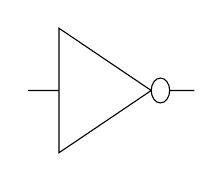
\begin{tikzpicture}[x=0.75pt,y=0.75pt,yscale=-1,xscale=1]
					\draw   (61.81,42) -- (106.26,72) -- (61.81,102) -- (61.81,42) -- cycle (47,72) -- (61.81,72) (115.15,72) -- (127,72) (106.26,72) .. controls (106.26,68.69) and (108.25,66) .. (110.7,66) .. controls (113.16,66) and (115.15,68.69) .. (115.15,72) .. controls (115.15,75.31) and (113.16,78) .. (110.7,78) .. controls (108.25,78) and (106.26,75.31) .. (106.26,72) -- cycle ;
				\end{tikzpicture}
				\vfill \null    
				\columnbreak
				\begin{center}
					\begin{tabular}{c|c}
						A & B \\ \hline
						0 & 1 \\
						1 & 0 
					\end{tabular}
				\end{center}
				\vfill \null    
				\columnbreak
				\begin{center}
					~\\
					\fbox{$B = \bar{A}$}
				\end{center}
				\vfill \null    
				\columnbreak
			\end{multicols}
		}
		
		\item{AND Gate}
		\subitem{
			
			\begin{multicols}{3}
				\tikzset{every picture/.style={line width=0.75pt}} %set default line width to 0.75pt        
				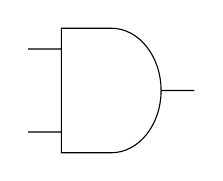
\begin{tikzpicture}[x=0.75pt,y=0.75pt,yscale=-1,xscale=1]
					
					\draw   (61.81,41) -- (85.81,41) .. controls (99.06,41) and (109.81,54.44) .. (109.81,71) .. controls (109.81,87.56) and (99.06,101) .. (85.81,101) -- (61.81,101) -- (61.81,41) -- cycle (45.81,51) -- (61.81,51) (45.81,91) -- (61.81,91) (109.81,71) -- (125.81,71) ;
				\end{tikzpicture}
				\vfill \null    
				\columnbreak
				\begin{center}
					\begin{tabular}{c|c|c}
						A & B & C \\ \hline
						0 & 0 & 0 \\
						0 & 1 & 0 \\
						1 & 0 & 0 \\
						1 & 1 & 1 \\				
					\end{tabular}
				\end{center}
				\vfill \null    
				\columnbreak
				\begin{center}
					~\\
					\fbox{$B = A . B $}
				\end{center}
				\vfill \null    
				\columnbreak
			\end{multicols}	
			
		}
		\item{OR Gate}
		\subitem{
			\begin{multicols}{3}
				\tikzset{every picture/.style={line width=0.75pt}} %set default line width to 0.75pt        
				
				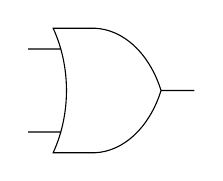
\begin{tikzpicture}[x=0.75pt,y=0.75pt,yscale=-1,xscale=1]
					%uncomment if require: \path (0,138); %set diagram left start at 0, and has height of 138
					
					%Shape: Or Gate [id:dp7848185808932866] 
					\draw   (61,41) -- (81,41) .. controls (94.95,41.54) and (107.42,53.23) .. (113,71) .. controls (107.42,88.77) and (94.95,100.46) .. (81,101) -- (61,101) .. controls (69.57,82.44) and (69.57,59.56) .. (61,41) -- cycle (49,51) -- (65,51) (49,91) -- (65,91) (113,71) -- (129,71) ;
				\end{tikzpicture}
				\vfill \null    
				\columnbreak
				\begin{center}
					\begin{tabular}{c|c|c}
						A & B & C \\ \hline
						0 & 0 & 0 \\
						0 & 1 & 0 \\
						1 & 0 & 0 \\
						1 & 1 & 1 \\				
					\end{tabular}
				\end{center}
				\vfill \null    
				\columnbreak
				\begin{center}
					~\\
					\fbox{$C = A + B $}
				\end{center}
				\vfill \null    
				\columnbreak
			\end{multicols}	
			
			
			
	}	\end{enumerate}
	\newpage
	\subsection{Advanced Logic Gates}
	
	\begin{enumerate}
		
		
		\item{NOR Gate}
		\subitem{
			
			\begin{multicols}{3}
				\tikzset{every picture/.style={line width=0.75pt}} %set default line width to 0.75pt        
				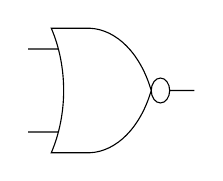
\begin{tikzpicture}[x=0.75pt,y=0.75pt,yscale=-1,xscale=1]
					\draw   (62.48,41) -- (81,41) .. controls (93.92,41.54) and (105.47,53.23) .. (110.63,71) .. controls (105.47,88.77) and (93.92,100.46) .. (81,101) -- (62.48,101) .. controls (70.42,82.44) and (70.42,59.56) .. (62.48,41) -- cycle (51.37,51) -- (66.19,51) (51.37,91) -- (66.19,91) (119.52,71) -- (131.37,71) (110.63,71) .. controls (110.63,67.69) and (112.62,65) .. (115.07,65) .. controls (117.53,65) and (119.52,67.69) .. (119.52,71) .. controls (119.52,74.31) and (117.53,77) .. (115.07,77) .. controls (112.62,77) and (110.63,74.31) .. (110.63,71) -- cycle ;
				\end{tikzpicture}
				
				
				\begin{center}
					\begin{tabular}{c|c|c}
						A & B & C \\ \hline
						0 & 0 & 1 \\
						0 & 1 & 0 \\
						1 & 0 & 0 \\
						1 & 1 & 0 \\				
					\end{tabular}
				\end{center}
				\vfill \null    
				\columnbreak
				\begin{center}
					~\\
					\fbox{$B = \overline{A+B} $}
				\end{center}
				\vfill \null    
				\columnbreak
			\end{multicols}	
			
		}
		
		\item{NAND Gate}
		\subitem{
			
			\begin{multicols}{3}
				\tikzset{every picture/.style={line width=0.75pt}} %set default line width to 0.75pt         
				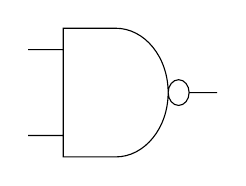
\begin{tikzpicture}[x=0.75pt,y=0.75pt,yscale=-1,xscale=1] 
					\draw   (64.85,38) -- (90.13,38) .. controls (104.08,38) and (115.41,51.89) .. (115.41,69) .. controls (115.41,86.11) and (104.08,100) .. (90.13,100) -- (64.85,100) -- (64.85,38) -- cycle (48,48.33) -- (64.85,48.33) (48,89.67) -- (64.85,89.67) (125.52,69) -- (139,69) (115.41,69) .. controls (115.41,65.58) and (117.67,62.8) .. (120.46,62.8) .. controls (123.26,62.8) and (125.52,65.58) .. (125.52,69) .. controls (125.52,72.42) and (123.26,75.2) .. (120.46,75.2) .. controls (117.67,75.2) and (115.41,72.42) .. (115.41,69) -- cycle ;		
				\end{tikzpicture}
				\vfill \null    
				\columnbreak
				\begin{center}
					\begin{tabular}{c|c|c}
						A & B & C \\ \hline
						0 & 0 & 1 \\
						0 & 1 & 1 \\
						1 & 0 & 1 \\
						1 & 1 & 0 \\				
					\end{tabular}
				\end{center}
				\vfill \null    
				\columnbreak
				\begin{center}
					~\\
					\fbox{$B = \overline{A.B} $}
				\end{center}
				\vfill \null    
				\columnbreak
			\end{multicols}	
			
		}
		\item{XOR Gate}
		\subitem{
			\begin{multicols}{3}
				
				\tikzset{every picture/.style={line width=0.75pt}} %set default line width to 0.75pt        
				
				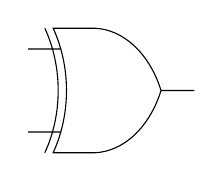
\begin{tikzpicture}[x=0.75pt,y=0.75pt,yscale=-1,xscale=1] 
					\draw   (54,38) -- (74,38) .. controls (87.95,38.54) and (100.42,50.23) .. (106,68) .. controls (100.42,85.77) and (87.95,97.46) .. (74,98) -- (54,98) .. controls (62.57,79.44) and (62.57,56.56) .. (54,38) -- cycle (42,48) -- (58,48) (42,88) -- (58,88) (106,68) -- (122,68) (50,38) .. controls (58.57,56.56) and (58.57,79.44) .. (50,98) ;			
				\end{tikzpicture}
				
				\vfill \null    
				\columnbreak
				\begin{center}
					\begin{tabular}{c|c|c}
						A & B & C \\ \hline
						0 & 0 & 0 \\
						0 & 1 & 1 \\
						1 & 0 & 1 \\
						1 & 1 & 0 \\				
					\end{tabular}
				\end{center}
				\vfill \null    
				\columnbreak
				\begin{center}
					~\\
					\fbox{$C = A \oplus B $}
				\end{center}
				\vfill \null    
				\columnbreak
			\end{multicols}		
		}
	\end{enumerate}
	\newpage
	\section{Laws of Boolean Algebra}
	\begin{itemize}
		\item{\underline{Associative Law}}
		\subitem{
			
			
			\tcbset{
				enhanced,
				colback=red!5!white,
				boxrule=0.1pt,
				colframe=black!75!black,
				fonttitle=\bfseries
			}
			
			\begin{center}
				\begin{tcolorbox}[center title,    %%<<---- here
					lifted shadow={1mm}{-2mm}{3mm}{0.1mm}%
					{black!50!white}]
					\abovedisplayskip=0pt% <--- remove vertical space above align
					\belowdisplayskip=0pt% <--- remove vertical space below align
					\begin{varwidth}{\textwidth}
						\begin{align*}
							(A+B) + C          & = A+(B+C)             \\
							(A \cdot B)\cdot C & = A \cdot (B \cdot C) 
						\end{align*}
					\end{varwidth}
				\end{tcolorbox}
			\end{center}
		}
		\bigskip
		\bigskip
		\item{\underline{Commutative Law}}
		\subitem{
			\tcbset{
				enhanced,
				colback=red!5!white,
				boxrule=0.1pt,
				colframe=black!75!black,
				fonttitle=\bfseries
			}
			\begin{center}
				\begin{tcolorbox}[center title,    %%<<---- here
					lifted shadow={1mm}{-2mm}{3mm}{0.1mm}%
					{black!50!white}]
					\abovedisplayskip=0pt% <--- remove vertical space above align
					\belowdisplayskip=0pt% <--- remove vertical space below align
					\begin{varwidth}{\textwidth}
						\begin{align*}
							A+B       & = B+A       \\
							A \cdot B & = B \cdot A 
						\end{align*}
					\end{varwidth}
				\end{tcolorbox}
				
			\end{center}
			
		}
		\bigskip
		\bigskip
		\item{\underline{Distributive Law}}
		\subitem{
			\tcbset{
				enhanced,
				colback=red!5!white,
				boxrule=0.1pt,
				colframe=black!75!black,
				fonttitle=\bfseries
			}
			\begin{center}
				\begin{tcolorbox}[center title,    %%<<---- here
					lifted shadow={1mm}{-2mm}{3mm}{0.1mm}%
					{black!50!white}]
					\abovedisplayskip=0pt% <--- remove vertical space above align
					\belowdisplayskip=0pt% <--- remove vertical space below align
					\begin{varwidth}{\textwidth}
						\begin{align*}
							A+(B \cdot C)   & = (A \cdot B) + (A \cdot C) \\
							A \cdot (B + C) & = (A+ B) \cdot (A + C)      
						\end{align*}
					\end{varwidth}
				\end{tcolorbox}
				
			\end{center}
			
		}
		\bigskip
		\bigskip
		\item{\underline{Tautology Law}}
		\subitem{
			\tcbset{
				enhanced,
				colback=red!5!white,
				boxrule=0.1pt,
				colframe=black!75!black,
				fonttitle=\bfseries
			}
			\begin{center}
				\begin{tcolorbox}[center title,    %%<<---- here
					lifted shadow={1mm}{-2mm}{3mm}{0.1mm}%
					{black!50!white}]
					\abovedisplayskip=0pt% <--- remove vertical space above align
					\belowdisplayskip=0pt% <--- remove vertical space below align
					\begin{varwidth}{\textwidth}
						\begin{align*}
							A+A       & = A & \qquad A + \bar{A}     & = 1 \\	
							A \cdot A & = A & \qquad	A \cdot \bar{A} & =\O 
						\end{align*}
					\end{varwidth}
				\end{tcolorbox} 
			\end{center}
		}
		\bigskip
		\bigskip
		\item{\underline{Common Sense Law}}
		\subitem{
			\tcbset{
				enhanced,
				colback=red!5!white,
				boxrule=0.1pt,
				colframe=black!75!black,
				fonttitle=\bfseries
			}
			\begin{center}
				\begin{tcolorbox}[center title,    %%<<---- here
					lifted shadow={1mm}{-2mm}{3mm}{0.1mm}%
					{black!50!white}]
					\abovedisplayskip=0pt% <--- remove vertical space above align
					\belowdisplayskip=0pt% <--- remove vertical space below align
					\begin{varwidth}{\textwidth}
						\begin{align*}
							A+1       & = 1 & \qquad A + \O     & = A \\	
							A \cdot 1 & = A & \qquad	A \cdot \O & =\O 
						\end{align*}
					\end{varwidth}
				\end{tcolorbox} 
			\end{center}
		}
		\newpage
		\item{\underline{Absorption Law}}
		\subitem{
			\tcbset{
				enhanced,
				colback=red!5!white,
				boxrule=0.1pt,
				colframe=black!75!black,
				fonttitle=\bfseries
			}
			\begin{center}
				\begin{tcolorbox}[center title,    %%<<---- here
					lifted shadow={1mm}{-2mm}{3mm}{0.1mm}%
					{black!50!white}]
					\abovedisplayskip=0pt% <--- remove vertical space above align
					\belowdisplayskip=0pt% <--- remove vertical space below align
					\begin{varwidth}{\textwidth}
						\begin{align*}
							A + (A \cdot B)     & = A \\	
							A \cdot (A \cdot B) & = A 
						\end{align*}
					\end{varwidth}
				\end{tcolorbox} 
			\end{center}
		}
		\item{\underline{Double Complement Law}}
		\subitem{
			\tcbset{
				enhanced,
				colback=red!5!white,
				boxrule=0.1pt,
				colframe=black!75!black,
				fonttitle=\bfseries
			}
			\begin{center}
				\begin{tcolorbox}[center title,    %%<<---- here
					lifted shadow={1mm}{-2mm}{3mm}{0.1mm}%
					{black!50!white}]
					\abovedisplayskip=0pt% <--- remove vertical space above align
					\belowdisplayskip=0pt% <--- remove vertical space below align
					\begin{varwidth}{\textwidth}
						\begin{align*}
							\bar{\bar{A}} =                                        & A                                                    \\
							\overline{\bar{A} \cdot \bar{B}} \neq A \cdot B  \quad & ; \quad \overline{(\overline{A\cdot B})} = A \cdot B 
						\end{align*}
					\end{varwidth}
				\end{tcolorbox} 
			\end{center}
		}
		\item{\underline{De Morgan's Law}}
		\subitem{
			\tcbset{
				enhanced,
				colback=red!5!white,
				boxrule=0.1pt,
				colframe=black!75!black,
				fonttitle=\bfseries
			}
			\begin{center}
				\begin{tcolorbox}[center title,    %%<<---- here
					lifted shadow={1mm}{-2mm}{3mm}{0.1mm}%
					{black!50!white}]
					\abovedisplayskip=0pt% <--- remove vertical space above align
					\belowdisplayskip=0pt% <--- remove vertical space below align
					\begin{varwidth}{\textwidth}
						\begin{align*}
							\bar{A} + \bar{B}     & =\overline{A \cdot B} \\
							\bar{A} \cdot \bar{B} & = \overline{A + B}    
						\end{align*}
					\end{varwidth}
				\end{tcolorbox} 
			\end{center}
		}
		
	\end{itemize}
	\subsection{Exercises}
	\begin{example}
		Simplify $\bar{A} \cdot \bar{B} + A \cdot \bar{B} + \bar{A} \cdot B$
	\end{example}
	\begin{alignat*}{2}
		&   &        & \bar{A}\cdot\bar{B} + A\cdot B + \bar{A} \cdot B \\
		&   & =\quad & \bar{B}\cdot(\bar{A}\cdot A) + (\bar{A} \cdot B) \\
		&   & =\quad & (\bar{B} \cdot 1) + (\bar{A} \cdot B)            \\
		&   & =\quad & \bar{B} + (\bar{A} \cdot B)                      \\
		&   & =\quad & (\bar{B}+\bar{A})  \cdot (\bar{B}+B)             \\
		&   & =\quad & (\bar{B}+\bar{A}) \cdot 1                        \\
		&   & =\quad & \overline{(A+B)} \quad                           
	\end{alignat*}
	\hrulefill
	\newpage
	\begin{example}
		Prove that $A \cdot B + A \cdot \bar{B}  \cdot C+A = A$
	\end{example}
	\begin{alignat*}{2}
		&   &        & A \cdot B + A \cdot \bar{B}  \cdot C+A = A \\
		&   & =\quad & A \cdot(B+ \bar{B} \cdot C + 1)            \\
		&   & =\quad & A  \cdot ( (C \cdot 1)  + 1 )              \\
		&   & =\quad & A \cdot (C+1)                              \\
		&   & =\quad & A                                          
	\end{alignat*}
	\hrulefill
	\begin{example}
		Simplify $ABC + \bar{A}BC+A\bar{B}C + AB\bar{C}$
	\end{example}
	\begin{alignat*}{2}
		&   &        & ABC + \bar{A}BC+A\bar{B}C + AB\bar{C}                 \\
		&   & =\quad & BC \cdot (A+\bar{A}) + A\bar{B}C + AB\bar{C}          \\
		&   & =\quad & B(C+A\bar{C}) + A\bar{B} C                            \\
		&   & =\quad & B\left((A+C)\cdot (C + \bar{C}) \right) + A\bar{B}  C \\
		&   & =\quad & B(A+C) + A\bar{B} C                                   \\
		&   & =\quad & BC + AB + A\bar{B} C                                  \\
		&   & =\quad & BC + A(B+(B\cdot C))                                  \\
		&   & =\quad & BC + A\left((B+\bar{B}) \cdot(B+C)\right)             \\
		&   & =\quad & AB + AC + BC                                          
	\end{alignat*}
	\hrulefill
	\newpage
	\section{Applications of Logic Gates}
	\subsection{BCD to Gray Code Convertor}
	\paragraph{Problem:}
	Develop a logic circuit which takes in 4 inputs in BCD format and returns a Gray Code equivalent in 4-bits.
	\begin{center}
		\begin{tabular}{c|c|c|c|c||c|c|c|c}
			& \multicolumn{4}{c|}{BCD} & \multicolumn{4}{c|}{Gray Code} \\ \hline
			DEC & A & B & C & D & W & X & Y & Z \\ \hline
			0   & 0 & 0 & 0 & 0 & 1 & 1 & 1 & 0 \\ \hline
			1   & 0 & 0 & 0 & 1 & 0 & 0 & 1 & 0 \\ \hline
			2   & 0 & 0 & 1 & 0 & 1 & 0 & 1 & 1 \\ \hline
			3   & 0 & 0 & 1 & 1 & 1 & 0 & 1 & 1 \\ \hline
			4   & 0 & 1 & 0 & 0 & 0 & 1 & 1 & 1 \\ \hline
			5   & 0 & 1 & 0 & 1 & 1 & 1 & 0 & 1 \\ \hline
			6   & 0 & 1 & 1 & 0 & 1 & 1 & 0 & 1 \\ \hline
			7   & 0 & 1 & 1 & 1 & 1 & 0 & 1 & 0 \\ \hline
			8   & 1 & 0 & 0 & 0 & 1 & 1 & 1 & 1 \\ \hline
			9   & 1 & 0 & 0 & 1 & 1 & 1 & 1 & 1 \\ \hline
			10  & \multicolumn{8}{c|}{DON'T CARE}                           \\ 
		\end{tabular}
	\end{center}
	\begin{multicols}{2}
		\begin{center}
			$W=$	\begin{4kmap}{AB}{CD}
				\contingut{0,0,1,X,0,0,1,X,0,0,X,X,0,0,X,X}	
				\implicant{3}{10}{red}
			\end{4kmap}
		\end{center}
		\begin{center}
			$Y=$	\begin{4kmap}{AB}{CD}
				\contingut{0,1,0,X,0,1,0,X,1,0,X,X,1,0,X,X}
				\implicantedges{12}{10}{red}
				\implicant{1}{7}{green}
			\end{4kmap}
		\end{center}
		\begin{center}
			$X=$	\begin{4kmap}{AB}{CD}
				\contingut{0,1,1,X,0,1,1,X,0,1,X,X,0,1,X,X}
				\implicant{1}{11}{red}
				\implicant{3}{10}{yellow}
			\end{4kmap}
		\end{center}
		\begin{center}
			$Z=$	\begin{4kmap}{AB}{CD}
				\contingut{0,0,0,X,1,1,1,X,1,1,X,X,0,0,X,X}
				\implicant{4}{6}{red}
				\implicant{8}{10}{blue}
			\end{4kmap}
		\end{center}
		
	\end{multicols}
	\begin{multicols}{2}
		\begin{center}
			$W = A$
		\end{center}
	
	
		\begin{center}
			$Y = B\oplus C$
		\end{center}
	
	
		\begin{center}
			$X = A + B$
		\end{center}	
	
	
		\begin{center}
			$Z = C\oplus D$
		\end{center}	
		
		
		
		
		
	\end{multicols}
	\newpage
	\subsection{7-Segment LED Display}
	\paragraph*{Problem: }
	Develop a logic circuit that returns the state of the $A$ segment inside a 1-digit 7-segment LED display.
	
	\begin{multicols}{2}
		\begin{center}
			\begin{tabular}{c||c|c|c|c||c|c|c|c|c|c|c}
				DEC & W & X & Y & Z & A & B & C & D & E & F & G \\ \hline
				0   & 0 & 0 & 0 & 0 & 1 & 1 & 1 & 0 & 1 & 1 & 1 \\ \hline
				1   & 0 & 0 & 0 & 1 & 0 & 0 & 1 & 0 & 0 & 1 & 0 \\ \hline
				2   & 0 & 0 & 1 & 0 & 1 & 0 & 1 & 1 & 1 & 0 & 1 \\ \hline
				3   & 0 & 0 & 1 & 1 & 1 & 0 & 1 & 1 & 0 & 1 & 1 \\ \hline
				4   & 0 & 1 & 0 & 0 & 0 & 1 & 1 & 1 & 0 & 1 & 0 \\ \hline
				5   & 0 & 1 & 0 & 1 & 1 & 1 & 0 & 1 & 0 & 1 & 1 \\ \hline
				6   & 0 & 1 & 1 & 0 & 1 & 1 & 0 & 1 & 1 & 1 & 1 \\ \hline
				7   & 0 & 1 & 1 & 1 & 1 & 0 & 1 & 0 & 0 & 1 & 0 \\ \hline
				8   & 1 & 0 & 0 & 0 & 1 & 1 & 1 & 1 & 1 & 1 & 1 \\ \hline
				9   & 1 & 0 & 0 & 1 & 1 & 1 & 1 & 1 & 0 & 1 & 1 \\ \hline
				10       & \multicolumn{11}{c|}{\multirow{2}{*}{DON'T CARE}} \\ \cline{1-1}
				$\vdots$ & \multicolumn{11}{c|}{}                            \\ \hline
			\end{tabular}
			~\\
			\begin{alignat*}{2}
				&   & A & = \overline{\bar{W}X\bar{Y}\bar{Z} + \bar{W}\bar{X}\bar{Y}Z} \\
				&   &   & = (W+\bar{X}+Y+Z)\cdot (W+X+Y+\bar{Z})                       
			\end{alignat*}
			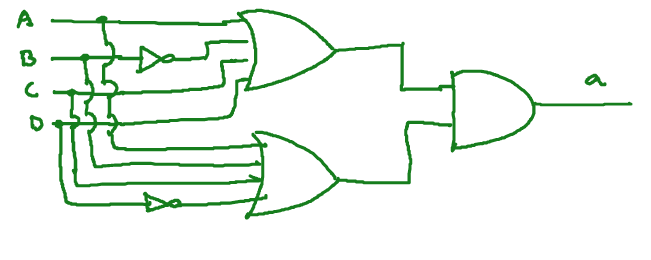
\includegraphics[scale=0.5]{a7SEG}
		\end{center}
		\begin{center}
			~\\~\\
			\qquad\qquad\qquad\qquad\qquad	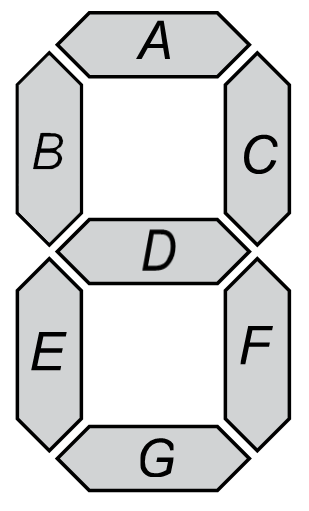
\includegraphics[scale=0.3]{7seg}
			
		\end{center}
		\qquad\qquad\qquad\qquad $A=$\begin{4kmap}{WX}{YZ}
			\contingut{1,0,1,X,0,1,1,X,1,1,X,X,1,1,X,X}
			\implicantsol{1}{red}
			\implicantsol{4}{yellow}
		\end{4kmap}
	\end{multicols}
	
	
	
	
	\newpage
	\subsection{Comparator}
	\paragraph*{Problem: }
	Develop a logic circuit that can be used to compare two 2-bit binary numbers $x, y$. The circuit should be able to detect if $x<y$ , $x=y$ or $x>y$. Label your output: Less than (L), Equal (E), Greater than (G).
	
	\begin{center}
		\begin{tabular}{c|c|c|c||c|c|c}
			$A$ & $B$ & $C$ & $D$ & L & E & G \\ \hline
			0   & 0   & 0   & 0   & 0 & 1 & 0 \\ \hline
			0   & 0   & 0   & 1   & 1 & 0 & 0 \\ \hline
			0   & 0   & 1   & 0   & 1 & 0 & 0 \\ \hline
			0   & 0   & 1   & 1   & 1 & 0 & 0 \\ \hline
			0   & 1   & 0   & 0   & 0 & 0 & 1 \\ \hline
			0   & 1   & 0   & 1   & 0 & 1 & 0 \\ \hline
			0   & 1   & 1   & 0   & 1 & 0 & 0 \\ \hline
			0   & 1   & 1   & 1   & 1 & 0 & 0 \\ \hline
			1   & 0   & 0   & 0   & 0 & 0 & 1 \\ \hline
			1   & 0   & 0   & 1   & 0 & 0 & 1 \\ \hline
			1   & 0   & 1   & 0   & 0 & 1 & 0 \\ \hline
			1   & 0   & 1   & 1   & 1 & 0 & 0 \\ \hline
			1   & 1   & 0   & 0   & 0 & 0 & 1 \\ \hline
			1   & 1   & 0   & 1   & 0 & 0 & 1 \\ \hline
			1   & 1   & 1   & 0   & 0 & 0 & 1 \\ \hline
			1   & 1   & 1   & 1   & 0 & 1 & 0 
		\end{tabular}
	\end{center}
	\begin{center}
		$ x = A B$, $y = C D$\\
	\end{center}
	\begin{multicols}{3}
		\begin{center}
			\begin{4kmap}{AB}{CD}
				\contingut{0,0,0,0,1,0,0,0,1,1,0,0,1,1,1,0}
				\implicant{4}{12}{yellow}
				\implicantedges{12}{14}{green}
				\implicant{12}{9}{purple}
			\end{4kmap}\\
			$L = \bar{A}C + \bar{A} \bar{B} D + \bar{B} CD$
		\end{center}
		\begin{center}
			\begin{4kmap}{AB}{CD}
				\contingut{1,0,0,0,0,1,0,0,0,0,1,0,0,0,0,1}
				\implicantsol{0}{purple}
				\implicantsol{5}{purple}
				\implicantsol{15}{purple}
				\implicantsol{10}{purple}
			\end{4kmap}\\
			$E = (B\odot D)\cdot (A\odot C)$
		\end{center}
		\begin{center}
			\begin{4kmap}{AB}{CD}
				\contingut{0,1,1,1,0,0,1,1,0,0,0,1,0,0,0,0}
				\implicanttopdown{3}{11}{red}
				\implicant{3}{6}{blue}
				\implicant{1}{3}{yellow}
			\end{4kmap}\\
			$G = A\bar{C} + B\bar{C}\bar{D} + AB\bar{D}$
		\end{center}
	\end{multicols}
\newpage
\subsection{S\&M to Two's Complement Converter}
\paragraph{Problem: }If $A_2A_1A_0$ is a 3 bit sign and magnitude binary number and $B_2B_1B_0$ is a 3 bit 2's Complement number draw the Karnaugh maps of $B_2B_1B_0$ in terms of $A_2A_1A_0$ and hence obtain the minimized boolean expression for  $B_2B_1B_0$.

\begin{center}
\begin{tabular}{c|c|c|c||c|c|c}
	Decimal & \multicolumn{3}{c||}{S\&M} & \multicolumn{3}{c}{2's Comp.} \\ \hline
	& $A_2$   & $A_1$  & $A_0$  & $B_2$    & $B_1$    & $B_0$    \\ \hline
	+0      & 0       & 0      & 0      & 0        & 0        & 0        \\ \hline
	1       & 0       & 0      & 0      & 0        & 0        & 1        \\ \hline
	2       & 0       & 0      & 1      & 0        & 1        & 0        \\ \hline
	3       & 0       & 0      & 1      & 0        & 1        & 1        \\ \hline
	-0      & 0       & 1      & 0      & X        & X        & X        \\ \hline
	-1      & 1       & 0      & 1      & 1        & 1        & 1        \\ \hline
	-2      & 1       & 1      & 0      & 1        & 1        & 0        \\ \hline
	-3      & 1       & 1      & 1      & 1        & 0        & 1       
\end{tabular}
\end{center}~\\
\begin{multicols}{3}
	\begin{center}
$B_2=$	\begin{24kmap}{$A_2A_1$}{$A_0$}
		\contingut{0,0,X,1,0,0,1,1}
		\implicant{3}{6}{red}
	\end{24kmap}
\end{center}
\begin{center}
	$B_1=$	\begin{24kmap}{$A_2A_1$}{$A_0$}
		\contingut{0,1,X,1,0,1,1,0}
		\implicant{1}{3}{red}
		\implicant{1}{5}{blue}
		\implicant{2}{6}{green}
	\end{24kmap}
\end{center}
\begin{center}
	$B_0=$\begin{24kmap}{$A_2A_1$}{$A_0$}
		\contingut{0,0,X,0,1,1,1,1}
		\implicant{4}{6}{red}
	\end{24kmap}
\end{center}
\end{multicols}
\newpage
\subsection{Multiplexer}
\paragraph*{Problem: } If two 4-bit numbers are input to the multiplexer and a select line (to inputs $A$ and $B$) can be high or low, develop a multiplexer such that the inputs A are switched on to the output when the select line is high otherwise B is switched when the select line is low.\\ 
\begin{center}
	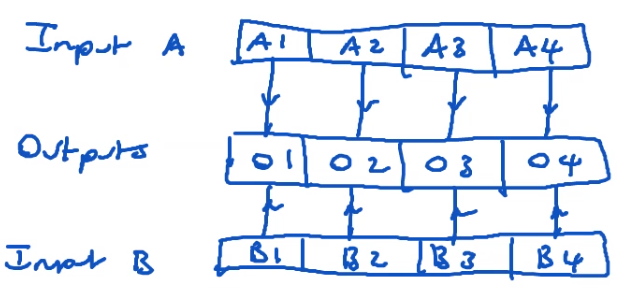
\includegraphics[scale=0.5]{multiplexer}
	
\end{center}

\newpage
\subsection{2-bit Binary Adder}
Consider two binary numbers $X_1X_2$ and $Y_1Y_2$. Assume they are added and the result had to be outputted from a logic circuit. Develop a logic circuit which performs this process.
\begin{center}
\begin{tabular}{c|c|c|c||c|c|c}
	$X_1$ & $X_2$ & $Y_1$ & $Y_2$ & $A$ & $B$ & $C$ \\ \hline
	0     & 0     & 0     & 0     & 0   & 0   & 0   \\ \hline
	0     & 0     & 0     & 1     & 0   & 0   & 1   \\ \hline
	0     & 0     & 1     & 0     & 0   & 1   & 0   \\ \hline
	0     & 0     & 1     & 1     & 0   & 1   & 1   \\ \hline
	0     & 1     & 0     & 0     & 0   & 0   & 1   \\ \hline
	0     & 1     & 0     & 1     & 0   & 1   & 0   \\ \hline
	0     & 1     & 1     & 0     & 0   & 1   & 1   \\ \hline
	0     & 1     & 1     & 1     & 1   & 0   & 0   \\ \hline
	1     & 0     & 0     & 0     & 0   & 1   & 0   \\ \hline
	1     & 0     & 0     & 1     & 0   & 1   & 1   \\ \hline
	1     & 0     & 1     & 0     & 1   & 0   & 0   \\ \hline
	1     & 0     & 1     & 1     & 1   & 0   & 1   \\ \hline
	1     & 1     & 0     & 0     & 0   & 1   & 1   \\ \hline
	1     & 1     & 0     & 1     & 1   & 0   & 0   \\ \hline
	1     & 1     & 1     & 0     & 1   & 0   & 1   \\ \hline
	1     & 1     & 1     & 1     & 1   & 1   & 1  
\end{tabular}
\end{center}
\begin{multicols}{3}
	\begin{center}
		\begin{4kmap}{$X_1X_2$}{$Y_1Y_2$}
			\contingut{0,0,0,0,0,0,0,1,0,0,1,1,0,1,1,1}
			\implicant{15}{10}{red}
			\implicant{7}{15}{blue}
			\implicant{13}{15}{black}
		\end{4kmap}
	$A = X_1X_2Y_2 + X_2Y_1Y_2 + X_1Y_1$
	\end{center}
	\begin{center}
	\begin{4kmap}{$X_1X_2$}{$Y_1Y_2$}
		\contingut{0,0,1,1,0,1,1,0,1,1,0,0,1,0,0,1}
		\implicantsol{5}{red}
		\implicantsol{15}{yellow}
		\implicant{3}{2}{green}
		\implicant{2}{6}{purple}
		\implicant{12}{8}{blue}
		\implicant{8}{9}{black}
	\end{4kmap}

$B = \bar{X_1}X_2\bar{Y_1}Y_2  + X_1X_2Y_1Y_2 + \bar{X_1}\bar{X_2}Y_1 + Y_1\bar{Y_2}\bar{X_1}X_2 $\\
$+ \bar{Y_1}\bar{Y_2}X_1 + X_1\bar{X_2}\bar{Y_1}$
	\end{center}
\begin{center}
\end{center}
\end{multicols}
\subsection{Odd Parity Check}
\paragraph*{Problem: } A 3-bit binary code is to be used to transmit information from point A to point B. As a check on the information received, a parity check is to be used. If odd parity is to be used, develop a circuit which can be used to add the parity bit  at the transmitting end and a separate circuit which can be used to check parity at the receiving end.
\begin{center}
\begin{tabular}{c|c|c||c}
	A & B & C & P \\ \hline
	0 & 0 & 0 & 1 \\ \hline
	0 & 0 & 1 & 0 \\ \hline
	0 & 1 & 0 & 0 \\ \hline
	0 & 1 & 1 & 1 \\ \hline
	1 & 0 & 0 & 0 \\ \hline
	1 & 0 & 1 & 1 \\ \hline
	1 & 1 & 0 & 1 \\ \hline
	1 & 1 & 1 & 0
\end{tabular}
\end{center}


\subsection{Panel Display Fuel}
\paragraph*{Problem: } A panel display has five lamps $L_1, L_2, L_3, L_4, L_5$ such that they indicate the level of fuel in the tank. The level-sensing circuit produces a binary number from zero to ten to represent the fuel level, where zero indicates "no fuel" and ten indicates "full tank".
\begin{center}
	\begin{tabular}{|c|l|}
		\hline
		Level Reading & \multicolumn{1}{c|}{Lamps Lit} \\ \hline
		0 to 2        & $L_1$                          \\ \hline
		3 to 4        & $L_1, L_2$                     \\ \hline
		5 to 6        & $L_1, L_2, L_3$                \\ \hline
		7  to 8       & $L_1, L_2, L_3, L_4$           \\ \hline
		9 to 10       & $L_1, L_2, L_3, L_4, L_5$      \\ \hline
		1             & \multicolumn{1}{c|}{0}         \\ \hline
		1             & \multicolumn{1}{c|}{1}         \\ \hline
		1             & \multicolumn{1}{c|}{1}         \\ \hline
	\end{tabular}
\end{center}
\end{document}